\section{Result}
\label{Result}
9 MCP PMTs were tested in testing system. The mean and standard deviation of parameters are calculated and shown in following sections.

\subsection{Gain, single PE resolution, P/V ratio, rise time, fall time and FWHM}
% \begin{figure}[!htbp]
%     \centering
%     \begin{subfigure}[b]{0.49\textwidth}
%         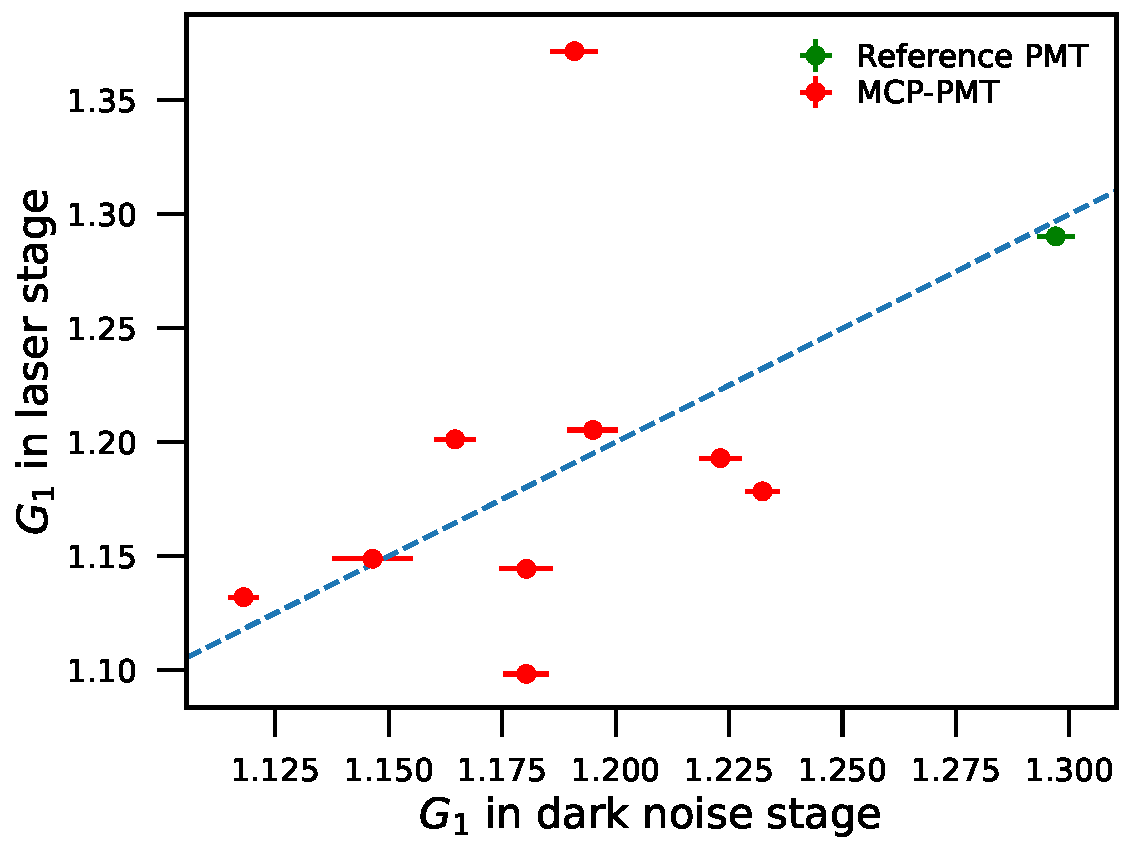
\includegraphics[width=\textwidth,page=1]{figures/result/compare.pdf}
%         \caption{}
%         \label{fig:gainCompare}
%     \end{subfigure}
%     \begin{subfigure}[b]{0.49\textwidth}
%         \includegraphics[width=\textwidth,page=2]{figures/result/compare.pdf}
%         \caption{}
%         \label{fig:speresolutionCompare}
%     \end{subfigure}
%     \caption{(a) Gain of main peak of PMTs for noise and trigger stage. (b) Resolution of main peak for noise and trigger stage}
% \end{figure}
% Fig.~\ref{fig:gainCompare} indicates that the gainof noise stage and trigger stage are consistent.
Due to the rate of trigger stage is larger than noise stage, the weight of pedestal in noise stager is larger than that of trigger stage.
% Fig.~\ref{fig:speresolutionCompare} shows 
Single PE resolution of trigger stage is better than that of noise stage due to a larger weight of the pedestal in noise stage smear the main peak of charge distribution. Due to the pedestal in dark noise stage has an obvious influence on $\mu_{C_t}$, the distribution of $\mu_{C_t}$ is not shown. Fig.~\ref{fig:totalchargeCompare} shows that mean of total charge $\mu_{C_t}$ is about 2 times of gain of main peak, which should be considered in reconstruction. Althogth the resolution of main peak of MCP-PMT is better than reference PMT, the long tail leads that the resolution of total charge is worse than reference PMT in Fig.~\ref{fig:totalchargeCompare}.

\begin{figure}[!htbp]
    \centering
    \includegraphics[width=0.5\textwidth,page=4]{figures/result/compare.pdf}
    \caption{Gain of single PE $\mu_{C_t}$ and resolution of single PE $\frac{\sigma_{C_t}}{\mu_{C_t}}$ for trigger stage.}
    \label{fig:totalchargeCompare}
\end{figure}

The ratio of pedestal also lead to the P/V ratio of trigger ratio is better than noise stage, as shown in Fig.~\ref{fig:PVCompare}.
\begin{figure}[!htbp]
    \centering
    \begin{subfigure}[b]{0.49\textwidth}
        \includegraphics[width=\textwidth,page=6]{figures/result/compare.pdf}
        \caption{}
        \label{fig:PVCompare}
    \end{subfigure}
    \begin{subfigure}[b]{0.49\textwidth}
        \includegraphics[width=\textwidth,page=7]{figures/result/compare.pdf}
        \caption{}
        \label{fig:RiseCompare}
    \end{subfigure}
    \caption{(a) P/V ratio. (b) Rise time, Fall time, and FWHM}
\end{figure}

As for time characteristics, the rise time, fall time, and FWHM are consistent between noise stage and trigger stage as shown in Fig.~\ref{fig:RiseCompare}.

\subsection{DCR, relative PDE, and TTS}
The dark count rate and relative PDE of different MCP-PMTs are show in Fig.~\ref{fig:DCRCompare}. The mean DCR and mean PDE are \SI{}{kHz} and .
\begin{figure}[!htbp]
    \centering
    \begin{subfigure}[b]{0.49\textwidth}
        \includegraphics[width=\textwidth,page=8]{figures/result/compare.pdf}
        \caption{}
        \label{fig:DCRCompare}
    \end{subfigure}
    \begin{subfigure}[b]{0.49\textwidth}
        \includegraphics[width=\textwidth,page=9]{figures/result/compare.pdf}
        \caption{}
        \label{fig:TTSCompare}
    \end{subfigure}
    \caption{(a) DCR vs PDE (b) TTS results}
\end{figure}

The TTS of different MCP-PMTs are show in Fig.~\ref{fig:TTSCompare}. The mean TTS is \SI{}{ns}.


\subsection{Pre-pulse and after-pulse}
\begin{figure}[!htbp]
    \centering
    \begin{subfigure}[b]{0.49\textwidth}
        \includegraphics[width=\textwidth,page=10]{figures/result/compare.pdf}
        \caption{}
        \label{fig:prepulseCompare}
    \end{subfigure}
    \begin{subfigure}[b]{0.49\textwidth}
        \includegraphics[width=\textwidth,page=11]{figures/result/compare.pdf}
        \caption{}
        \label{fig:afterpulseCompare}
    \end{subfigure}
    \caption{(a) pre-pulse ratio. (b) after-pulse ratio.}
\end{figure}
Ratio of pre-pulse and after-pulse is .
\begin{figure}[!htbp]
    \centering
    \begin{subfigure}[b]{0.49\textwidth}
        \includegraphics[width=\textwidth,page=13]{figures/result/compare.pdf}
        \caption{}
        \label{fig:afterpulsePeak}
    \end{subfigure}
    \begin{subfigure}[b]{0.49\textwidth}
        \includegraphics[width=\textwidth,page=12]{figures/result/compare.pdf}
        \caption{$\sigma$}
        \label{fig:sigmaCompare}
    \end{subfigure}
    \caption{(a) Time and ratio of peaks of after pulse ratio. (b) $\tau$ and $\sigma$}
\end{figure}

\subsection{Paramerters of SER}
The mean $\tau$ and $\sigma$ of SER is \SI{}{ns} and \SI{}{ns}.
\subsection{Energy resolution boost}

Assume the number of expected photons $N$ on PMT is $\mu_N$ and obey poisson distribution $\pi~(\mu_N)$. Energy $E$ of Event proportional to $N=k\eta E$, in which $k$ is the factor which is relate to light yield and light transportation and $eta$ is the PDE of PMT. The phton detection efficiency of PMT is $\eta$ and the sigle PE charge distribution is Gaussian distribution $G(\mu_c,\sigma_c)$. The output charge distribution $C$ is hierachical model and the expectation and variance are
\begin{align}
    E[C]&=\mu_N\mu_c\\
    Var[C]&=\mu_c^2\mu_N+\mu_N\sigma_c^2
\end{align}
To be convenience, $N$ is estimated as $\hat{N}=\frac{C}{\mu_c}$ and $E$ is estimated as $\hat{E}=\frac{\hat{N}}{k}$. For event of energy $E$, the reconstructed energy resolution is 
\begin{equation}
    \frac{\sqrt{Var[\hat{E}]}}{E[\hat{E}]}=\frac{\sqrt{\mu_c^2\mu_N+\mu_N\sigma_c^2}}{\mu_N\mu_c}=\frac{\sqrt{1+(\frac{\sigma_c}{\mu_c})^2}}{\sqrt{\mu_N}}=\frac{\sqrt{1+(\frac{\sigma_c}{\mu_c})^2}}{\sqrt{k\eta E}}
\end{equation}

The energy resolution is dominated by sigle PE charge distribution, which is illustrated in the Fig.~\ref{fig:EnergyResolution}. Althogh there exist a long tail in charge distribution of MCP-PMT, $\frac{\sigma_c}{\mu_c}$ of MCP-PMT is better than reference PMT.
\begin{figure}[!htbp]
    \centering
    \includegraphics[width=0.5\textwidth,page=14]{figures/result/compare.pdf}
    \caption{Energy resolution}
    \label{fig:EnergyResolution}
\end{figure}